\documentclass[]{beamer}
%\documentclass[handout]{beamer}
\usepackage{xmpmulti}
\usepackage{psfrag}
\usepackage{color}


\mode<presentation>
{
  \usetheme{Boadilla}  % very plain
}

\usepackage{xcolor}

\usepackage{amssymb,amsmath,amsthm}
\usepackage{boxedminipage}
\newcommand{\Expec}[2]{\mathbf{E}_{#1} \left[ #2 \right]}
\newcommand{\Prob}[2]{\mathbf{P}_{#1} \left( #2 \right)}



\title[]{Come Spedire un Diamante in Segreto}
\subtitle{Messaggi Privati con lo SmartPhone}

\author{Giuseppe Persiano}

\institute[UNISA]{%
Universit\`a di Salerno\\ \qquad \\
}

\date[Febbraio 2019] % (optional, should be abbreviation of conference name)
{25 Febbraio 2019}
% - Either use conference name or its abbreviation.

%\pgfdeclareimage[height=2.0cm]{university-logo}{sfu-vector-crest}
%\logo{\pgfuseimage{university-logo}}

\begin{document}

\newcommand{\zu}{\{0,1\}}
\newcommand{\ignore}[1]{}

\begin{frame}
  \titlepage
\end{frame}

%\section{Outline}
%\frame{\tableofcontents}

\ignore{
    \begin{frame}
    \frametitle{Outline}
    \tableofcontents
    % You might wish to add the option [pausesections]
    \end{frame}
}


\begin{frame}
\frametitle{Privacy delle comunicazioni}

\begin{block}{Booking e Repubblica}
\begin{itemize}
\item prenoto l'albergo per {\color{brown} Torino} usando {\color{magenta} Booking}
\item da quel momento in poi {\color{magenta} Repubblica}
mi mostra pubblicit\`a di eventi in {\color{brown} Piemonte}
\end{itemize}
\end{block}
\pause

\begin{center}
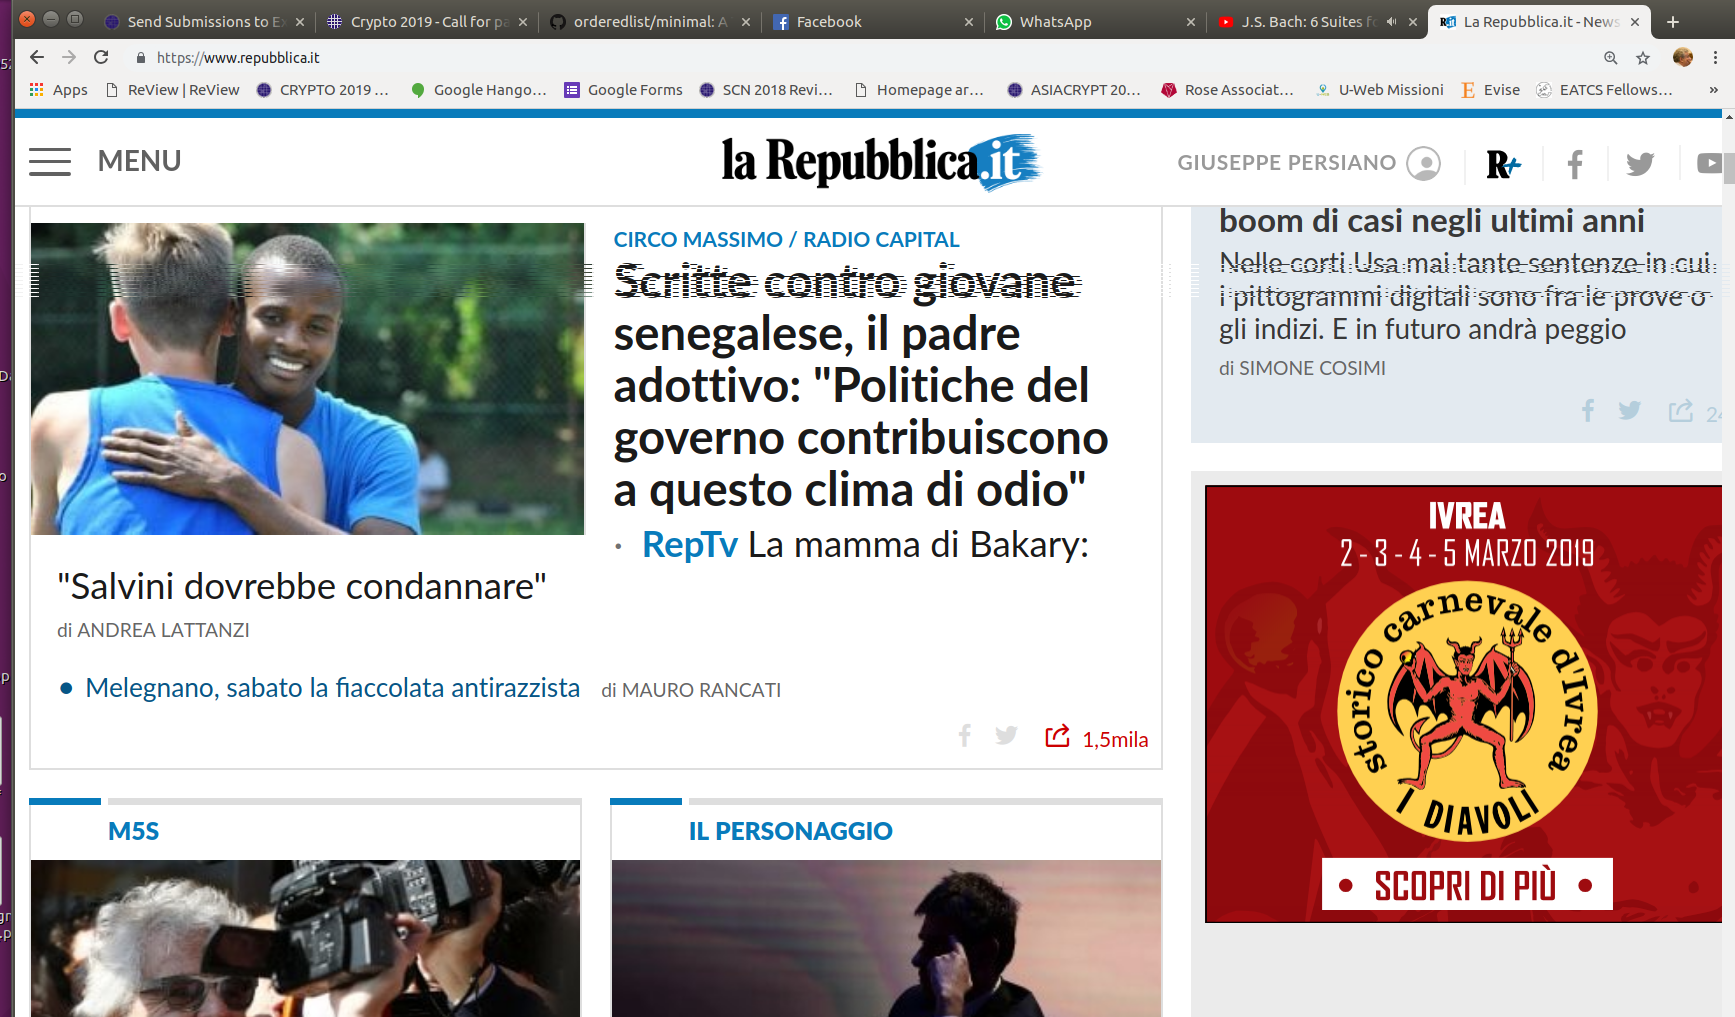
\includegraphics[width=3in]{Images/diamante/screenshot.png}
\end{center}
\end{frame}


\begin{frame}
\frametitle{Privacy delle comunicazioni}

\begin{block}{Facebook e Chrome}
\begin{itemize}
\item visito un sito di orologi
\item {\color{magenta} Facebook} inizia a presentarmi pubblicit\`a di orologi
\end{itemize}
\end{block}
\pause
\begin{block}{{\color{magenta} Gmail}}
\begin{itemize}
\item scambio email per accordarmi ad una visita di lavoro a {\color{brown} NYU}
\item pubblicit\`a per alberghi a {\color{brown} New York}
\end{itemize}
\end{block}
\pause

\vfill
\centerline{\alert{Whatsapp}???}
\end{frame}

\begin{frame}
\frametitle{Whatsapp usa end-to-end encryption}

{\color{brown} Anna vuole inviare un messaggio a Bernardo}

\begin{itemize}
\color{olive}
\item Il messaggio \`e cifrato dallo smart phone di Anna
\item Attraversa Internet fino a Bernardo in forma cifrato
\item Lo smart phone di Bernardo lo decifra
\end{itemize}

\pause

\vfill
\begin{center}
\color{brown}{Come \`e possibile?}
\end{center}
\end{frame}

\begin{frame}
\frametitle{Schemi di Cifratura}
Una coppia di algoritmi ${\color{magenta} (E,D)}$
$${\color{magenta} E(K,M)=C\qquad D(K,C)=M}$$

$$\begin{array}{ccc}
{\color{blue} K\in\zu^k} & 
{\color{blue} M\in\zu^m} & 
{\color{blue} C\in\zu^c} \\
{\color{brown} chiave} & 
{\color{brown} messaggio}& 
{\color{brown} crittogramma}
\end{array}
$$

\pause
\begin{enumerate}
\item {\color{magenta} A}({\color{green} nna}) sceglie ${\color{blue} K\in\zu^k}$
\item Cifra il file usando la chiave ${\color{blue} K}$
\item Conserva il file e la chiave in luoghi separati
\end{enumerate}
\end{frame}

\begin{frame}
\frametitle{Advanced Encryption Standard}

\begin{itemize}
\item Algoritmo \alert{pubblico} e utilizzabile gratuitamente
\pause
\item Scelto dopo una competizione scientifica durata dal 1997-2000
\begin{itemize}
{\color{blue}
\item Annuncio del Gennaio 1997
\item Richiesta ufficiale del Settembre 1997 per proposte di algoritmi di cifratura
\item 15 proposte iniziali da gruppi di ricercatori da tutto il mondo
\item 5 finalisti annunciati, Agosto 1999
\item Rijndael scelto ad Ottobre 2000 come {Advanced Encryption Standard} (AES)
}
\end{itemize}
\pause
\item Ratificato dal {\color{olive}\em National Institute of Standards and Technology}, USA
\pause
\item Chiave di 128, 192, 256 bit
\pause
\item Cifra blocchi di dati di 128 bit
\pause
\item Considerato sicuro dalla comunit\`a scientifica
\pause
\item Implementazioni disponibili: \alert{openssl.org}
\end{itemize}

\end{frame}

\ignore{
\begin{frame}
\frametitle{Esempio di Utilizzo con OpenSSL}
{\small 
{\tt
{\color{magenta} openssl aes-128-ecb} -e -K {\color{blue} 000102030405060708090A0B0C0D0E0F} -in {\color{red} voti.txt} -out {\color{red} votiCifrati.txt}
}}

\begin{itemize}
\item<2-> {\tt \color{magenta} openssl aes-128-ecb} 

Specifica il tipo di cifrario: 

\begin{itemize}
\item Advanced Encryption Standard ({\tt AES}) 
\item con chiave di 128 bit
\item in modalit\`a Electronic CodeBook  ({\tt ECB})
\end{itemize}

\item <3-> {\tt -e}

Specifica che il file deve essere cifrato ({\tt encrypted})

\item <4-> {\tt -K {\color{blue} 000102030405060708090A0B0C0D0E0F}}

Fornisce la chiave in esadecimale. 

Ogni carattere corrisponde a 4 bit.

\item <5->
{\tt -in {\color{red} voti.txt}}

Specifica il file di input.

\item <6->{\tt -out {\color{red} votiCifrati.txt}}

Specifica il file di output.
\end{itemize}
\end{frame}

\begin{frame}
\frametitle{Esempio di Utilizzo con OpenSSL 256 bit}
{\small 
{\tt
{\color{magenta} openssl aes-256-ecb} -e -K {\color{blue} 0000111122223333444455556666777788889999AAAABBBBCCCCDDDDEEEEFFFF} -in {\color{red} voti.txt} -out {\color{red} votiCifrati.txt}
}}

\begin{itemize}
\item{\tt \color{magenta} openssl aes-256-ecb} 

Specifica il tipo di cifrario: 

\begin{itemize}
\item Advanced Encryption Standard ({\tt AES}) 
\item con chiave di 256 bit
\item in modalit\`a Electronic CodeBook  ({\tt ECB})
\end{itemize}

\item{\tt -K {\small\color{blue} 0000111122223333444455556666777788889999AAAABBBBCCCCDDDDEEEEFFFF}}
Fornisce la chiave in esadecimale. 

Ogni carattere corrisponde a 4 bit.

\end{itemize}
\end{frame}

\begin{frame}

\only<1>{
\begin{tabular}{|p{3.5cm}||p{7.0cm}|}\hline
{\tt voti.txt} & {\tt votiCifrati.txt} \\ \hline\hline
{\tt AntonioArrigoni} &
{\tt e685e1f53302b52a747e0c5b10ae6374} \\
{\tt MarcelloRapetti} &
{\tt 460e01138bc583308c7dbc6512389e89} \\
{\tt CarmineTisognin} &
{\tt 691e95773c29d113c17ee3fccf22ece3} \\
{\tt CarmineTisognin} &
{\tt 691e95773c29d113c17ee3fccf22ece3} \\
{\tt GiacomoBunitaro} &
{\tt f54724a817b2c60c0d9581c13300091d} \\
{\tt CarmineTisognin} &
{\tt 691e95773c29d113c17ee3fccf22ece3} \\
{\tt AntonioArrigoni} &
{\tt e685e1f53302b52a747e0c5b10ae6374} \\
{\tt MarcelloRapetti} &
{\tt 460e01138bc583308c7dbc6512389e89} \\
{\tt AntonioArrigoni} &
{\tt e685e1f53302b52a747e0c5b10ae6374} \\
{\tt GiacomoBunitaro} &
{\tt f54724a817b2c60c0d9581c13300091d} \\
{\tt MarcelloRapetti} &
{\tt 460e01138bc583308c7dbc6512389e89}\\ \hline
\end{tabular}
}
\only<2>{
\begin{tabular}{|p{3.5cm}||p{7.0cm}|}\hline
{\tt voti.txt} & {\tt votiCifrati.txt} \\ \hline\hline
{\tt {\color{red} AntonioArrigoni}} &
{\tt {\color{red} e685e1f53302b52a747e0c5b10ae6374}} \\
{\tt MarcelloRapetti} &
{\tt 460e01138bc583308c7dbc6512389e89} \\
{\tt CarmineTisognin} &
{\tt 691e95773c29d113c17ee3fccf22ece3} \\
{\tt CarmineTisognin} &
{\tt 691e95773c29d113c17ee3fccf22ece3} \\
{\tt GiacomoBunitaro} &
{\tt f54724a817b2c60c0d9581c13300091d} \\
{\tt CarmineTisognin} &
{\tt 691e95773c29d113c17ee3fccf22ece3}\\
{\tt {\color{red} AntonioArrigoni}} &
{\tt {\color{red} e685e1f53302b52a747e0c5b10ae6374}} \\
{\tt MarcelloRapetti} &
{\tt 460e01138bc583308c7dbc6512389e89} \\
{\tt \color{red} AntonioArrigoni} &
{\tt \color{red} e685e1f53302b52a747e0c5b10ae6374} \\
{\tt GiacomoBunitaro} &
{\tt f54724a817b2c60c0d9581c13300091d} \\
{\tt MarcelloRapetti} &
{\tt 460e01138bc583308c7dbc6512389e89}\\ \hline
\end{tabular}
}
\only<3>{
\begin{tabular}{|p{3.5cm}||p{7.0cm}|}\hline
{\tt voti.txt} & {\tt votiCifrati.txt} \\ \hline\hline
{\tt \color{red} AntonioArrigoni} &
{\tt \color{red} e685e1f53302b52a747e0c5b10ae6374} \\
{\tt \color{blue} MarcelloRapetti} &
{\tt \color{blue} 460e01138bc583308c7dbc6512389e89} \\
{\tt CarmineTisognin} &
{\tt 691e95773c29d113c17ee3fccf22ece3} \\
{\tt CarmineTisognin} &
{\tt 691e95773c29d113c17ee3fccf22ece3} \\
{\tt GiacomoBunitaro} &
{\tt f54724a817b2c60c0d9581c13300091d} \\
{\tt CarmineTisognin} &
{\tt 691e95773c29d113c17ee3fccf22ece3} \\
{\tt \color{red} AntonioArrigoni} &
{\tt \color{red} e685e1f53302b52a747e0c5b10ae6374} \\
{\tt \color{blue} MarcelloRapetti} &
{\tt \color{blue} 460e01138bc583308c7dbc6512389e89} \\
{\tt \color{red} AntonioArrigoni} &
{\tt \color{red} e685e1f53302b52a747e0c5b10ae6374} \\
{\tt GiacomoBunitaro} &
{\tt f54724a817b2c60c0d9581c13300091d} \\
{\tt MarcelloRapetti} &
{\tt 460e01138bc583308c7dbc6512389e89}\\ \hline
\end{tabular}
}
\only<4>{
\begin{tabular}{|p{3.5cm}||p{7.0cm}|}\hline
{\tt voti.txt} & {\tt votiCifrati.txt} \\ \hline\hline
{\tt \color{red} AntonioArrigoni} &
{\tt \color{red} e685e1f53302b52a747e0c5b10ae6374} \\
{\tt \color{blue} MarcelloRapetti} &
{\tt \color{blue} 460e01138bc583308c7dbc6512389e89} \\
{\tt \color{green} CarmineTisognin} &
{\tt \color{green} 691e95773c29d113c17ee3fccf22ece3} \\
{\tt \color{green} CarmineTisognin} &
{\tt \color{green} 691e95773c29d113c17ee3fccf22ece3} \\
{\tt GiacomoBunitaro} &
{\tt f54724a817b2c60c0d9581c13300091d} \\
{\tt \color{green} CarmineTisognin} &
{\tt \color{green} 691e95773c29d113c17ee3fccf22ece3} \\
{\tt \color{red} AntonioArrigoni} &
{\tt \color{red} e685e1f53302b52a747e0c5b10ae6374} \\
{\tt \color{blue} MarcelloRapetti} &
{\tt \color{blue} 460e01138bc583308c7dbc6512389e89} \\
{\tt \color{red} AntonioArrigoni} &
{\tt \color{red} e685e1f53302b52a747e0c5b10ae6374} \\
{\tt GiacomoBunitaro} &
{\tt f54724a817b2c60c0d9581c13300091d} \\
{\tt MarcelloRapetti} &
{\tt 460e01138bc583308c7dbc6512389e89}\\ \hline
\end{tabular}
}
\end{frame}


\begin{frame}
\frametitle{Esempio di Utilizzo con OpenSSL}
{\small 
{\tt
{\color{magenta} openssl aes-128-cbc} -e -K {\color{blue} 000102030405060708090A0B0C0D0E0F} {\color{purple} -iv 0123456789ABCDEF} -in {\color{red} voti.txt} -out {\color{red} votiCBC.txt}
}}

\begin{itemize}
\item<2-> {\tt \color{magenta} openssl aes-128-cbc} 

Specifica il tipo di cifrario: 

\begin{itemize}
\item Advanced Encryption Standard ({\tt AES}) 
\item con chiave di 128 bit
\item in modalit\`a Cipher Block Chaining ({\tt CBC})
\end{itemize}
\item<3-> {\tt \color{purple} -iv 0123456789ABCDEF}

Valore dell'{\em Initialization Vector}
\end{itemize}
\end{frame}
}

\begin{frame}
\frametitle{Inviare messaggi privati}

{\color{red}Anna vuole mandare un messaggio privato a Bernardo}

\pause

\begin{itemize}
\color{magenta}
\item Anna cifra
\item Bernardo decifra
\end{itemize}

\pause

{\color{red} Ma con quale chiave?}

\begin{center}
\color{brown}
\em
La chiave usata per decifrare \alert{deve} essere la stessa usata per cifrare.
\end{center}

\pause
\vfill
{\color{blue} Anna e Bernardo si incontrano e si scambiano una chiavetta USB con la chiave}

\vfill
{\color{brown} Ideale per applicazioni militari}
\end{frame}

\begin{frame}
\frametitle{Inviare messaggi privati nell'era di WhatsApp}
{\color{magenta} ma anche Messenger, Telegram, Signal, Hangout,...}
\hfill
\includegraphics[width=1in]{Images/diamante/whatsapp.jpg}

\pause

\begin{block}{Key Agreement}
\begin{itemize}
{\color{blue}
\item Come fanno due persone che non si sono mai incontrate a scambiarsi
una chiave?
\pause
\item In modo privato, senza che nessuno la legga.
\pause
\item Un cane che si morde la coda:
\begin{itemize}
\item {\color{teal} se Anna e Bernardo possono scambiarsi una chiave in modo privato,
perch\'e non si scambiano direttamente il messaggio che voglio inviarsi?}
\end{itemize}
\pause
\item Ma \`e {\color{brown}\bf possibile}?
}
\end{itemize}
\end{block}
\end{frame}

\begin{frame}
\frametitle{Un problema simile}


\hfill
\includegraphics[width=1in]{Images/diamante/koohinoor.jpg}
\begin{block}{Come spedire un diamante}
\pause
\begin{itemize}
\color{blue}
\item <+-> Bernardo \`e in viaggio e compra un diamante per Anna.
\item <+-> Come pu\`o spedirglielo in maniera sicura?
\begin{itemize}
\color{teal}
\item <+-> Pu\`o metterlo in una cassaforte e chiuderla con un lucchetto.
\item <+-> Ed inviare la cassaforte e la chiave una con DHL e l'altra con
FedExp.
\item <+-> Funziona se i due corrieri non si mettono d'accordo...
\item <+-> O se nessuno intercetta i pacchi...
\end{itemize}
\item <+-> Possibile una soluzione che garantisce che nessuno pu\`o 
rubare il diamante?
\end{itemize}
\end{block}
\end{frame}

\begin{frame}
\frametitle{Un problema simile}
\begin{block}{Una soluzione}
\pause
\begin{itemize}
\color{blue}
\item <+-> Bernardo compra una cassaforte con {\color{red}\bf due} occhielli per lucchetto.
\item <+-> Bernardo mette il diamante nella cassaforte e un lucchetto in uno dei due occhielli. Tiene per s\'e la chiave del lucchetto.
\item <+-> Bernardo invia la cassaforte ad Anna.
\item <+-> Anna riceve la cassaforte e mette un lucchetto nell'occhiello libero.
Tiene per s\'e la chiave del lucchetto.
\item <+-> Anna invia la cassaforte a Bernardo.
\item <+-> Bernardo rimuove il suo lucchetto.
\item <+-> Bernardo invia la cassaforte ad Anna.
\item <+-> Anna riceve la cassaforte e usa la sua chiave per aprirla.
\end{itemize}
\end{block}
\end{frame}

\begin{frame}
\frametitle{Cosa succede???}

\begin{block}{La potenza della commutativit\`a}
\begin{itemize}
\item una cassaforta chiusa non pu\`o essere aperta senza la chiave
\item i lucchetti commutano:
    \begin{itemize}
    \item la cassaforte si apre anche se i lucchetti non sono rimossi nello
        stesso ordine
    \end{itemize}
\end{itemize}
\end{block}

\pause

\vfill

La moltiplicazione \`e commutativa!

$$x\cdot y=y\cdot x$$

\pause

\vfill
\begin{center}
{\color{magenta}
Cercasi cassaforte digitale che interagisca con moltiplicazione.
}
\end{center}

\end{frame}


\begin{frame}
\frametitle{Esponenziazione}
$$
\color{purple} (2^{x})^y=2^{x\cdot y}=(2^{y})^x$$

\pause

{\color{red} \`E una cassaforte sicura?
}

\pause

\vskip 1cm

\color{blue}
Non sugli interi...
\end{frame}

\begin{frame}
\frametitle{Diffie-Hellman }

Sia $p$ un primo.

\pause
\vskip 1cm
$\mathbb{Z}_p^\star$ \`e il gruppo degli interi $[1,\ldots,p-1]$
con moltiplicazione modulo $p$.

\pause
\vskip 1cm
$\mathbb{Z}_p^\star$ \`e un gruppo ciclico
\pause $\Rightarrow$
Esiste un \alert{generatore} $g$ t.c.:

$$\mathbb{Z}_p^\star=\{g^0,g^1,\ldots,g^{p-2}\}.$$

\pause

Ogni $a\in\mathbb{Z}_p^\star$ ha il \alert{\em logaritmo discreto}
\alert{\em in base $g$}.

$$x\ \text{\rm t.c.}\ a=g^x.$$

\end{frame}

\ignore{
\begin{frame}
\frametitle{Come verificare un generatore}

$5$ \`e un generatore di $\mathbb{Z}_p^\star$ per $p=47$.

Facile da verificare usando un semplice programmino in Sage:

\begin{block}{Verifica di un generatore}
{\tt 
def checkGenerator(p,gg):\\
\quad \\
    \quad K=GF(p)\\
    \quad g=K(gg)\\
    \quad num=[]\\
\quad \\
    \quad for x in range(p-1):\\
        \quad\quad  a=g\^{}x\\
        \quad\quad  if a in num:\\
            \quad\quad\quad   return False\\
        \quad\quad  num=num+[a]\\
\quad \\
    \quad return True
}
\end{block}
\end{frame}

\begin{frame}
\frametitle{Come calcolare il logaritmo discreto}

\begin{block}{Tabella del logaritmo discreto}
{\tt 
def printLogs(p,gg):\\
\quad    K=GF(p)\\
    \quad g=K(gg)         \\
    \quad logs=\{\}\\
    \quad for x in range(p-1):\\
        \quad\quad a=g\^{}x\\
        \quad \quad logs[a]=x\\
    \quad table=logs.keys()\\
    \quad table.sort()\\
    \quad for a in table:\\
        \quad\quad  print a,logs[a]
\quad \\

}

\end{block}
\end{frame}

\begin{frame}
\frametitle{Logaritmo discreto modulo 47 in base 5}
$$\begin{array}{|r|r||r|r||r|r||r|r|}
\hline
a & dlog & a & dlog & a & dlog & a & dlog \\\hline\hline

\input{dlog}

\hline
\end{array}$$

\end{frame}

\begin{frame}
\frametitle{Problema originario}

\begin{block}{Obiettivo}
Anna e Bernardo prima di mandare i messaggi cifrati
vogliono accordarsi su una chiave in modo privato
\end{block}
\end{frame}

\begin{frame}
\begin{block}{Scambio di Chiavi Diffie-Hellman (1978)}
\begin{enumerate}
\item Anna sceglie un primo $p$ e un generatore $g$ di $\mathbb{Z}_p^\star$;
\item Anna invia $p$ e $g$ a Bernardo;
\item Anna sceglie $a$ a caso in $[0,\ldots,p-2]$ e calcola $A=g^a$;
\item \alert{Anna invia $A$ a Bernardo;}
\item Bernardo sceglie $b$ a caso in $[0,\ldots,p-2]$ e calcola $B=g^b$;
\item \alert{Bernardo invia $B$ a Anna;}
\item Anna calcola $K_A=B^a$;
\item Bernardo calcola $K_B=A^b$;
\end{enumerate}
\end{block}

\pause

{\color{red} $$K_A=B^a=(g^b)^a=g^{b\cdot a}=g^{a\cdot b}=(g^a)^b=A^b=K_B$$}
\end{frame}
}

\begin{frame}
\frametitle{Esempio con $p=47$}

\begin{minipage}{6cm}
\begin{block}{Esempio in Sage}
{\tt \color{brown}
K=GF(47)\\
g=K(5)\\
{\color{blue}
a=K.random\_element()\\
A=g\^{}a\\
}
\quad \\
{\color{red}
b=K.random\_element()\\
B=g\^{}b\\
}
\quad \\
{\color{blue} print "Chiave calcolata da Anna",B\^{}a}\\
{\color{red} print "Chiave calcolata da Bernardo",A\^{}b}\\
}
\end{block}
\end{minipage}
\quad
\begin{minipage}{5cm}
\begin{block}{Esecuzione}
{\tt \color{blue}
Diffie Hellman con p = 47   e g = 5\\
\quad \\
a = 31    A = 39\\
\quad \\
b = 12    B = 18\\
\quad \\
Chiave calcolata da Anna 14\\
\quad \\
Chiave calcolata da Bernardo 14\\
}
\end{block}
\end{minipage}
\end{frame}

\ignore{

\begin{frame}
\frametitle{Quanto \`e forte la cassaforte?}

\begin{minipage}{9cm}
\begin{block}{}
\begin{itemize}
\item \alert{Anna invia $A=39$ a Bernardo;}
\item \alert{Bernardo invia $B=18$ a Anna;}
\item \alert{Carlo intercetta i due messaggi $A$}
\end{itemize}
\pause
{\color{blue}
Se Carlo potesse calcolare $a$ da $A$ potrebbe calcolare la chiave
come $B^a$.
}
\end{block}
\end{minipage}

\pause

\vskip 1cm
\begin{minipage}{7cm}
\begin{block}{}
{\tt\color{brown}
sage: K=GF(47) \\
sage: g=K(5) \\
sage: A=K(39) \\
sage: print discrete\_log(A,g) \\
31
}
\end{block}
\end{minipage}
\end{frame}
}
\begin{frame}
\frametitle{Scegliamo un primo pi\`u grande}

Il documento 
{\em Algorithms, Key Size and Protocols Report (2018)},
raccomanda $p$ di almeno 1024 bit. Per applicazioni con alto
livello di sicurezza almeno 3072 bit.



\begin{tabular}{rrrrrrrr}
{\tiny {\color{olive}\tt FFFFFFFF}} & {\tiny \color{olive}\tt FFFFFFFF} & {\tiny \color{olive}\tt C90FDAA2} & {\tiny \color{olive}\tt 2168C234} & {\tiny \color{olive}\tt C4C6628B} & {\tiny \color{olive}\tt 80DC1CD1} & {\tiny \color{olive}\tt 29024E08} & {\tiny \color{olive}\tt 8A67CC74} \\
{\tiny \color{olive}\tt 020BBEA6} & {\tiny \color{olive}\tt 3B139B22} & {\tiny \color{olive}\tt 514A0879} & {\tiny \color{olive}\tt 8E3404DD} & {\tiny \color{olive}\tt EF9519B3} & {\tiny \color{olive}\tt CD3A431B} & {\tiny \color{olive}\tt 302B0A6D} & {\tiny \color{olive}\tt F25F1437} \\
{\tiny \color{olive}\tt 4FE1356D} & {\tiny \color{olive}\tt 6D51C245} & {\tiny \color{olive}\tt E485B576} & {\tiny \color{olive}\tt 625E7EC6} & {\tiny \color{olive}\tt F44C42E9} & {\tiny \color{olive}\tt A637ED6B} & {\tiny \color{olive}\tt 0BFF5CB6} & {\tiny \color{olive}\tt F406B7ED} \\
{\tiny \color{olive}\tt EE386BFB} & {\tiny \color{olive}\tt 5A899FA5} & {\tiny \color{olive}\tt AE9F2411} & {\tiny \color{olive}\tt 7C4B1FE6} & {\tiny \color{olive}\tt 49286651} & {\tiny \color{olive}\tt ECE45B3D} & {\tiny \color{olive}\tt C2007CB8} & {\tiny \color{olive}\tt A163BF05} \\
{\tiny \color{olive}\tt 98DA4836} & {\tiny \color{olive}\tt 1C55D39A} & {\tiny \color{olive}\tt 69163FA8} & {\tiny \color{olive}\tt FD24CF5F} & {\tiny \color{olive}\tt 83655D23} & {\tiny \color{olive}\tt DCA3AD96} & {\tiny \color{olive}\tt 1C62F356} & {\tiny \color{olive}\tt 208552BB} \\
{\tiny \color{olive}\tt 9ED52907} & {\tiny \color{olive}\tt 7096966D} & {\tiny \color{olive}\tt 670C354E} & {\tiny \color{olive}\tt 4ABC9804} & {\tiny \color{olive}\tt F1746C08} & {\tiny \color{olive}\tt CA18217C} & {\tiny \color{olive}\tt 32905E46} & {\tiny \color{olive}\tt 2E36CE3B} \\
{\tiny \color{olive}\tt E39E772C} & {\tiny \color{olive}\tt 180E8603} & {\tiny \color{olive}\tt 9B2783A2} & {\tiny \color{olive}\tt EC07A28F} & {\tiny \color{olive}\tt B5C55DF0} & {\tiny \color{olive}\tt 6F4C52C9} & {\tiny \color{olive}\tt DE2BCBF6} & {\tiny \color{olive}\tt 95581718} \\
{\tiny \color{olive}\tt 3995497C} & {\tiny \color{olive}\tt EA956AE5} & {\tiny \color{olive}\tt 15D22618} & {\tiny \color{olive}\tt 98FA0510} & {\tiny \color{olive}\tt 15728E5A} & {\tiny \color{olive}\tt 8AAAC42D} & {\tiny \color{olive}\tt AD33170D} & {\tiny \color{olive}\tt 04507A33} \\
{\tiny \color{olive}\tt A85521AB} & {\tiny \color{olive}\tt DF1CBA64} & {\tiny \color{olive}\tt ECFB8504} & {\tiny \color{olive}\tt 58DBEF0A} & {\tiny \color{olive}\tt 8AEA7157} & {\tiny \color{olive}\tt 5D060C7D} & {\tiny \color{olive}\tt B3970F85} & {\tiny \color{olive}\tt A6E1E4C7} \\
{\tiny \color{olive}\tt ABF5AE8C} & {\tiny \color{olive}\tt DB0933D7} & {\tiny \color{olive}\tt 1E8C94E0} & {\tiny \color{olive}\tt 4A25619D} & {\tiny \color{olive}\tt CEE3D226} & {\tiny \color{olive}\tt 1AD2EE6B} & {\tiny \color{olive}\tt F12FFA06} & {\tiny \color{olive}\tt D98A0864} \\
{\tiny \color{olive}\tt D8760273} & {\tiny \color{olive}\tt 3EC86A64} & {\tiny \color{olive}\tt 521F2B18} & {\tiny \color{olive}\tt 177B200C} & {\tiny \color{olive}\tt BBE11757} & {\tiny \color{olive}\tt 7A615D6C} & {\tiny \color{olive}\tt 770988C0} & {\tiny \color{olive}\tt BAD946E2} \\
{\tiny \color{olive}\tt 08E24FA0} & {\tiny \color{olive}\tt 74E5AB31} & {\tiny \color{olive}\tt 43DB5BFC} & {\tiny \color{olive}\tt E0FD108E} & {\tiny \color{olive}\tt 4B82D120} & {\tiny \color{olive}\tt A93AD2CA} & {\tiny \color{olive}\tt FFFFFFFF} & {\tiny \color{olive}\tt FFFFFFFF} \\                     
\end{tabular}



\vfill

{\color{brown} \tt https://www.ietf.org/rfc/rfc3526.txt}

\end{frame}

\begin{frame}
\frametitle{Difficolt\`a del Logaritmo Discreto}

Il tempo per calcolare il logaritmo discreto dipende dalla lunghezza del modulo $p$.

\begin{itemize}
\item logaritmo discreto a 1024 bit richiede la potenza di calcolo di uno stato
\item logaritmo discreto a 3072 bit resta difficile da calcolare per i prossimi 30 anni
\end{itemize}

\end{frame}

\ignore{
\begin{frame}
\frametitle{ECDH}

$$y^2=x^3+486662\cdot x^2 + x\pmod 2^{255}-19\qquad\text{\rm Curve25519}$$

\begin{enumerate}
\item i punti di una curva ellittica costituiscono un gruppo ciclico
\item con un'operazione di ``addizione''
\item esponenziazione diventa moltiplicazione
\item possiamo eseguire Diffie-Hellman
\end{enumerate}

\begin{block}{ECDH}
{\tt\small E = EllipticCurve(GF(2\^{}255-19),[0,486662,0,1,0])}\\
{\tt\small G=E(9,14781619447589544791020593568}\\
{\tt\small \qquad 409986887264606134616475288964881837755586237401)}\\
{\tt\small p=E.order()}\\
{\tt\small a=int(Integers(p).random\_element());}\quad 
{\tt\small A=a*G}\\
{\tt\small b=int(Integers(p).random\_element());}\quad 
{\tt\small B=b*G}\\
{\tt\small KA=b*A}\\
{\tt\small KB=a*B}\\
\end{block}


\end{frame}
}

%%\begin{frame}
%%\frametitle{Quanto \`e forte la cassaforte?}
%%
%%\end{frame}

\begin{frame}
\frametitle{Whatsapp usa end-to-end encryption}

{\color{olive} Anna vuole inviare un messaggio a Bernardo}

\begin{itemize}
\color{brown}
\item Il messaggio \`e cifrato dallo smart phone di Anna
\item {\color{brown} Anna e Bernardo eseguono DH}
\begin{itemize}
\item {\color{brown} Condividono lo stesso intero $P$}
\end{itemize}

\item {\color{brown} Calcolano un hash di 256 bit di $P$ ed ottengono una chiave $K$ per AES a 256 bit}
\item {\color{brown} Anna cifra il messaggio }
\item Attraversa Internet fino a Bernardo in forma cifrato
\item Lo smart phone di Bernardo lo decifra
\item {\color{brown} Usando AES a 256 e chiave $K$}
\end{itemize}

\pause

\color{brown}{Versione semplificata!}
\end{frame}

\ignore{
\begin{frame}
\frametitle{Altri problemi da affrontare}

\begin{itemize}
\item Quando Anna esegue il protocollo per lo scambio della chiave come pu\`o essere sicura di parlare
    a Bernardo
\pause
\begin{itemize}
    \item Identificazione degli utenti
    \item Chiave pubblica basata su Curve Ellittiche
    \item Identit\`a garantita da Whatsapp
\end{itemize}
\pause
\item Supponiamo che Carlo ottenga la chiave usata per calcolare un messaggio

Pu\`o usare la chiave per decifrare i messaggi gi\`a inviati?
\pause
\begin{itemize}
    \item No. La chiave \`e  aggiornata ad ogni messaggio.
    \item Da una chiave non \`e possibile risalire alle chiavi precedenti.
\end{itemize}
\end{itemize}
\end{frame}
}

\begin{frame}
\frametitle{Morale della favola}
\pause
\begin{itemize}
\color{purple}
\item La riservatezza delle comunicazioni personali \`e importante ed \`e sotto attacco.
\pause
\item Esistono metodi {\em scientificamente} provati per proteggerli.
\pause
\item Esistono applicazioni che usano metodi {\em scientificamente} provati per proteggerli.
\pause
\item Alcune sono open-source
\begin{itemize}
\color{teal}
\item OpenSSL, Signal,...
\end{itemize}
\pause
\item Basati su matematica avanzata con cui possiamo sperimentare usando Sage.
\pause
\begin{itemize}
\color{teal}
\item Sage \`e open source e gratuito.
\end{itemize}
\end{itemize}
\end{frame}

\end{document}
